I trained each mode on the 347 GTEx + 601 TCGA samples with $\sim 20,000$ genes as features.
I trained each model on a random split of 77\% of the data, I then tested the accuracy of the trained models on the test data with the following results (Table \ref{ta}).
Clearly the models preformed well so I had some confidence in moving forward, but this is likely some kind of overfitting due to how many features were used.
% accuracy
\begin{table}[h]
    \centering
    \begin{tabular}{@{}ll@{}}
        \toprule
        Model & Test Accuracy \\
        \midrule
        SVM & 0.9937888198757764\\
        Naive Bayes & 0.9503105590062112\\
        Random Forest & 0.9968944099378882\\
        \bottomrule
    \end{tabular}
    \caption{Model accuracy on 33\% test set of transcriptomic data for healthy/cancerous lung cells.}
    \label{ta}
\end{table}
\FloatBarrier
% Gene Table
\begin{table}[h]
    \centering
    \begin{tabular}{@{}cllll@{}}
        \toprule
        & \multicolumn{4}{c}{Method} \\
        \cmidrule(l){2-5}
        Rank & SVM & Naive Bayes & Random Forest & $log_2$ Fold Change \\
        \midrule
        1 & ENSG00000198938.2  & ENSG00000198804.2  & ENSG00000188269.8  & ENSG00000134193.14\\
        2 & ENSG00000115414.18 & ENSG00000168878.16 & ENSG00000160013.8  & ENSG00000150244.11\\
        3 & ENSG00000019582.14 & ENSG00000198886.2  & ENSG00000047648.21 & ENSG00000147381.11\\
        4 & ENSG00000254709.7  & ENSG00000075624.13 & ENSG00000018280.16 & ENSG00000221867.8\\
        5 & ENSG00000086548.8  & ENSG00000185303.15 & ENSG00000206047.2  & ENSG00000170373.8\\
        \bottomrule
    \end{tabular}
    \caption{Most important genes (features) for each model as well as the most differentially expressed genes (largest $log_2$ fold change and adjusted p-value $< 0.05$)}
    \label{tb}
\end{table}
\FloatBarrier
Here Table \ref{tb} shows the genes that had the largest importance values for each model as well as the most differentially expressed genes.
I keep the DE genes here as they provide an intuitive reference for what genes should be good for training a binary classifier on this data.
It is interesting to note that there is no overlap among any of the models or even the DE genes, indicating that they all found different ways to accurately solve the classification problem.
After looking up online it appears that many of these genes are related to generating energy (cytochromes and cytoskeletal rearrangement (cell adhesion, fibronectin) which may be related to tumor growth and expansion.
However outliers like an olfactory receptor and prostoglandin are also present, so perhaps there is some issues with my pre-processing of the data.

% Distributions
\FloatBarrier
\begin{figure}[htb!]
    \center
    \makebox[\textwidth][c]{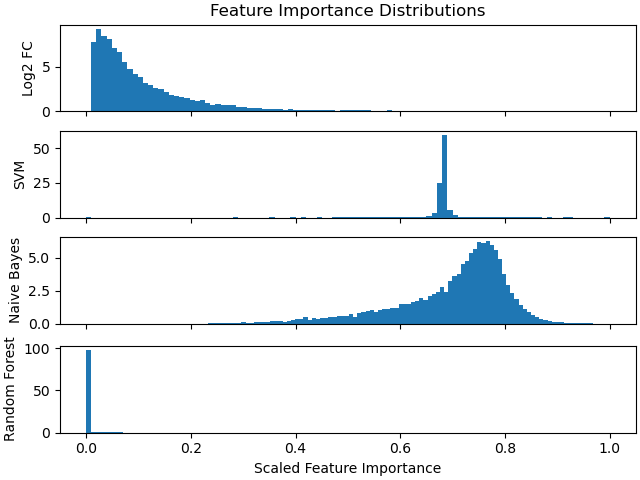
\includegraphics[width=0.7\linewidth]{../figures/importance_distributions.png}}
    \caption{Distribution of feature importances scaled to [0,1] for each model. For Log2 FC the absolute log fold change is show for genes that are differential expressed in cancer (adjusted p-value < 0.05)}
    \label{dist}
\end{figure}
\FloatBarrier
I find Figure \ref{dist} very interesting as even how many important genes or the average importance of genes are starkly different between the models.
It makes sense for Naive Bayes as a distribution is estimated for each gene, so the genes all posses some level of importance, but clearly there are some outliers of both highly influential and highly inflectional genes
The random forest distribution is also somewhat intuitive as in many cancer there are only a handful of genes that actually drive the growth of cancer and undergo large changes in expression.
This also lines up with the DE results since only about $\sim 4000$ genes were significantly differential expressed with a fold change $> 2$.
% Gene Upset
\FloatBarrier
\begin{figure}[htb!]
    \center
    \makebox[\textwidth][c]{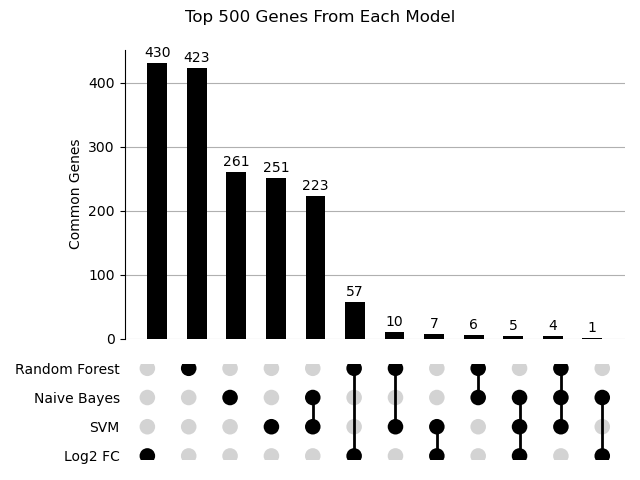
\includegraphics[width=0.5\linewidth]{../figures/upset_genes_500.png}}
    \caption{Upset plot of the top 500 most important genes for each model. For Log2 FC the absolute log fold change is show for genes that are differential expressed in cancer (adjusted p-value < 0.05)}
    \label{ugene}
\end{figure}
\FloatBarrier
% GO Upset
\FloatBarrier
\begin{figure}[htb!]
    \center
    \makebox[\textwidth][c]{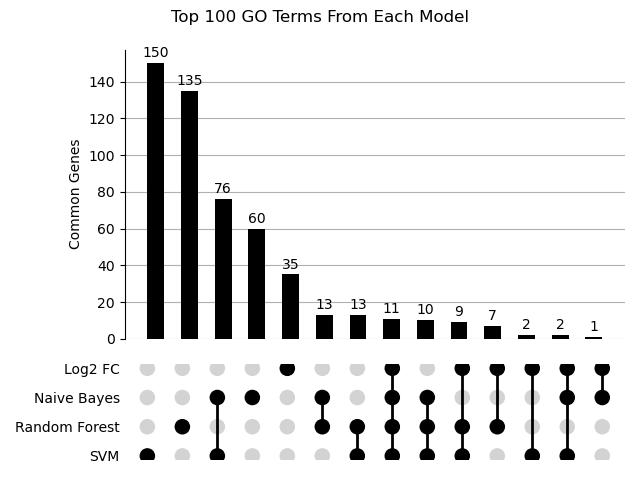
\includegraphics[width=0.5\linewidth]{../figures/upset_GO_100.png}}
    \caption{Upset plot of all GO terms associated with the top 100 most important genes for each model. For Log2 FC the absolute log fold change is show for genes that are differential expressed in cancer (adjusted p-value < 0.05)}
    \label{ugo}
\end{figure}
\FloatBarrier
Again in Figure \ref{ugene} and\ref{ugo} both show that the models have very little in common in terms of what genes they deemed important, but there are at least a few genes that all the models found.\footnote{Note that this is an upset plot, an alternative to a venn diagram, all categories are mutually exclusive, if you wish to know more \href{https://www.ncbi.nlm.nih.gov/pmc/articles/PMC4720993/}{here} is link to the publication.}
It is especially curios to see that 4 genes were prioritized by all 3 models but were not among the most differentially expressed genes.
% HeatMap
\FloatBarrier
\begin{figure}[htb!]
    \center
    \makebox[\textwidth][c]{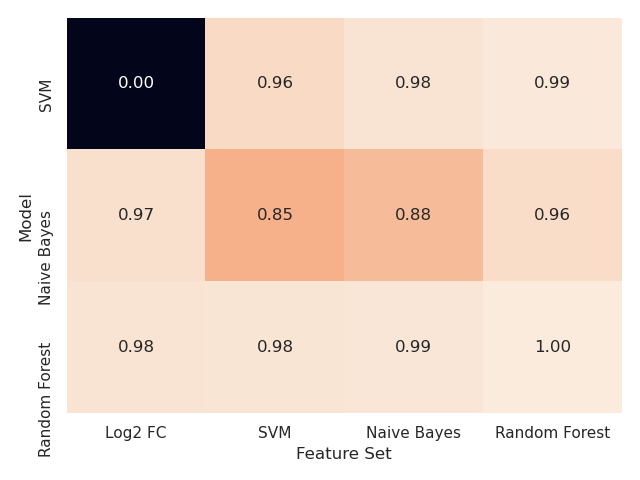
\includegraphics[width=0.7\linewidth]{../figures/heatmap.png}}
    \caption{Accuracy on the test data (n=322) for each model trained on the top 50 most important genes as determined by the trained model for the feature set. So the top 50 most important genes for SVM, when used to train a Naive Bayes Classifier, has an accuracy of 0.85. The top 50 absolute log2 fold change genes with adjusted p-value < 0.05 were also used as a feature set.}
    \label{heat}
\end{figure}
\FloatBarrier
Finally I tried to train each model on the top 50 most important genes found by each other model or by DE.
And despite the minimal overlap in what genes the models prioritize it seems like they are all capable of learning well from each other, save for Naive Bayes which appears to be lagging a little.
I would expect that this is because Naive Bayes is less robust to noise due to considering all features in classification, which is not necessarily true for the SVM or random forest.
Note that the SVM cell is 0 because the model failed to converge.
It is also possible that 50 genes is too many for 947 samples and may still be overfitting.

